\documentclass{article}
\usepackage[utf8]{inputenc}
\usepackage{amsfonts}
\usepackage{amssymb}
\usepackage{graphicx}
\usepackage{hyperref}
\usepackage{amsmath}
\usepackage{pgfplots}
\pgfplotsset{compat=1.18}
\usepackage[backend=biber, style=numeric]{biblatex}
\addbibresource{references.bib}
\usepackage{titlesec}
\titleformat{\subsection}[hang]{\normalfont\bfseries}{\thesubsection}{1em}{}
\usepackage{abstract}
\usepackage[labelformat=empty]{caption}

\begin{document}
\pagenumbering{gobble}
\begin{figure}
  \centering
  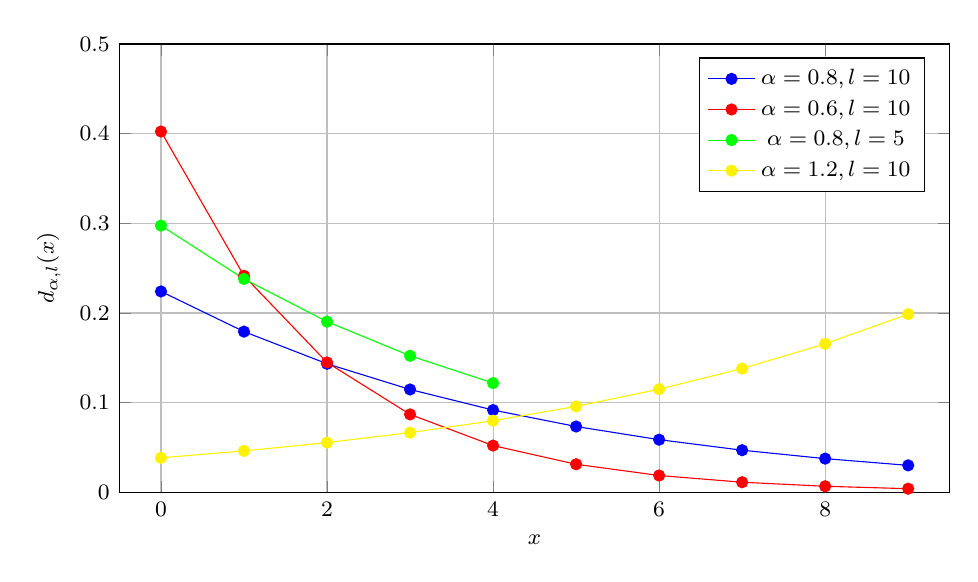
\begin{tikzpicture}
    \begin{axis}[
      xlabel={$x$},
      ylabel={$d_{\alpha, l}(x)$},
      xmin=-0.5, xmax=9.5,
      ymin=0, ymax=0.5,
      xtick={0,2,4,6,8,10},
      ytick={0,0.1,0.2,0.3,0.4,0.5},
      legend pos=north east,
      grid=major,
      width=\columnwidth,
      height=0.6\columnwidth,
      tick label style={font=\footnotesize},
      label style={font=\footnotesize},
      legend style={font=\footnotesize},
    ]
    
    \addplot[domain=0:9, samples=10, color=blue, mark=*]{0.8^x / ((1 - 0.8^10) / (1 - 0.8))};
    \addlegendentry{$\alpha = 0.8, l = 10$}
    
    \addplot[domain=0:9, samples=10, color=red, mark=*]{0.6^x / ((1 - 0.6^10) / (1 - 0.6))};
    \addlegendentry{$\alpha = 0.6, l = 10$}
    
    \addplot[domain=0:4, samples=5, color=green, mark=*]{0.8^x / ((1 - 0.8^5) / (1 - 0.8))};
    \addlegendentry{$\alpha = 0.8, l = 5$}

    \addplot[domain=0:9, samples=10, color=yellow, mark=*]{1.2^x / ((1 - 1.2^10) / (1 - 1.2))};
    \addlegendentry{$\alpha = 1.2, l = 10$}

    \end{axis}
  \end{tikzpicture}
  \caption{Geometric LDF with various parameter choices}
  \label{fig:geometric_ldf}
\end{figure}

\end{document}